%! TeX program = lualatex
%---------------------------ALLGEMEINE IMPORTS-------------------------------------
\documentclass[12pt,english,ngerman]{scrartcl}

%\input{./protokoll_template/template.latex/input/shared_preamble.tex}

    % Kopfzeile
\ihead{SS22\\11.11.2022}
\chead{\textsc{Stark} Matthias - 12004907 \\ \textsc{Philipp} Maximilian - 11839611}
\ohead{FLAB 1 \\ Zählrohr}
    % Fußzeile

\begin{document}
%\includepdf{}
\tableofcontents
\newpage

\section{Aufgabenstellung\label{Auf}}

\begin{itemize}
    \item Messung der $\alpha$, $\beta$ und $\gamma$ Strahlung ohne und mit verschiedenen dicken Abschirmungen
    \item Aufnahme der Zählrohrcharakteristik
    \item Aufnahme der Zählstatistik
    \item Bestätigung des Abstandsgesetzes
    \item Bestimmung der Endpunktsenergie über Absorbtion
    \item Aufnahme des Energiespektrums von $\beta$ Strahlung mit Magnetspektrometer
    \item Aufnahme und Kalibrierung des $\gamma$ Spektrums
    \item Aufnahme des komplexen $\gamma$ Spektrums und seinen Zerfallsprodukten
\end{itemize}

\section{Grundlagen}\label{Grund}


\section{Versuchsanordnung}\label{sec:Versuchsanordnung}

Im Laufe des Versuchs wurden 3 verschiedene Aufbauten verwendet die im Verlauf modifiziert wurden.

\subsection{Digitalzähler}\label{aufbau_Digz}

Für die ersten 4 Teile des Versuchs wird folgender Versuchsaufbau aus \autoref{fig:digz} realisiert.
Dabei wird das Präparat in die dafür vorgesehene Halterung geschoben, hinter der sich das Zählrohr befindet, 
welches mit dem Digitalzähler verbunden ist, wodurch ein einfaches Ablesen der Counts ermöglicht wird.
Auf der optischen Bank kann der Abstand zwischen Präparat und Zählrohr variiert und abgelesen werden.
Dabei ist zu beachten, dass die abgelesene Distanz auf der optischen Bank nicht dem tatsächlichen Abstand zwischen 
Probe und Zählrohr entspricht, da sich diese nicht direkt über den Sockel befinden. Um im späteren Verlauf des Versuchs die 
Aluminiumbleche zu befestigen, wird die entsprechende Halterung auf die optische Bank gesteckt.

\begin{figure}[H]
    \begin{center}
		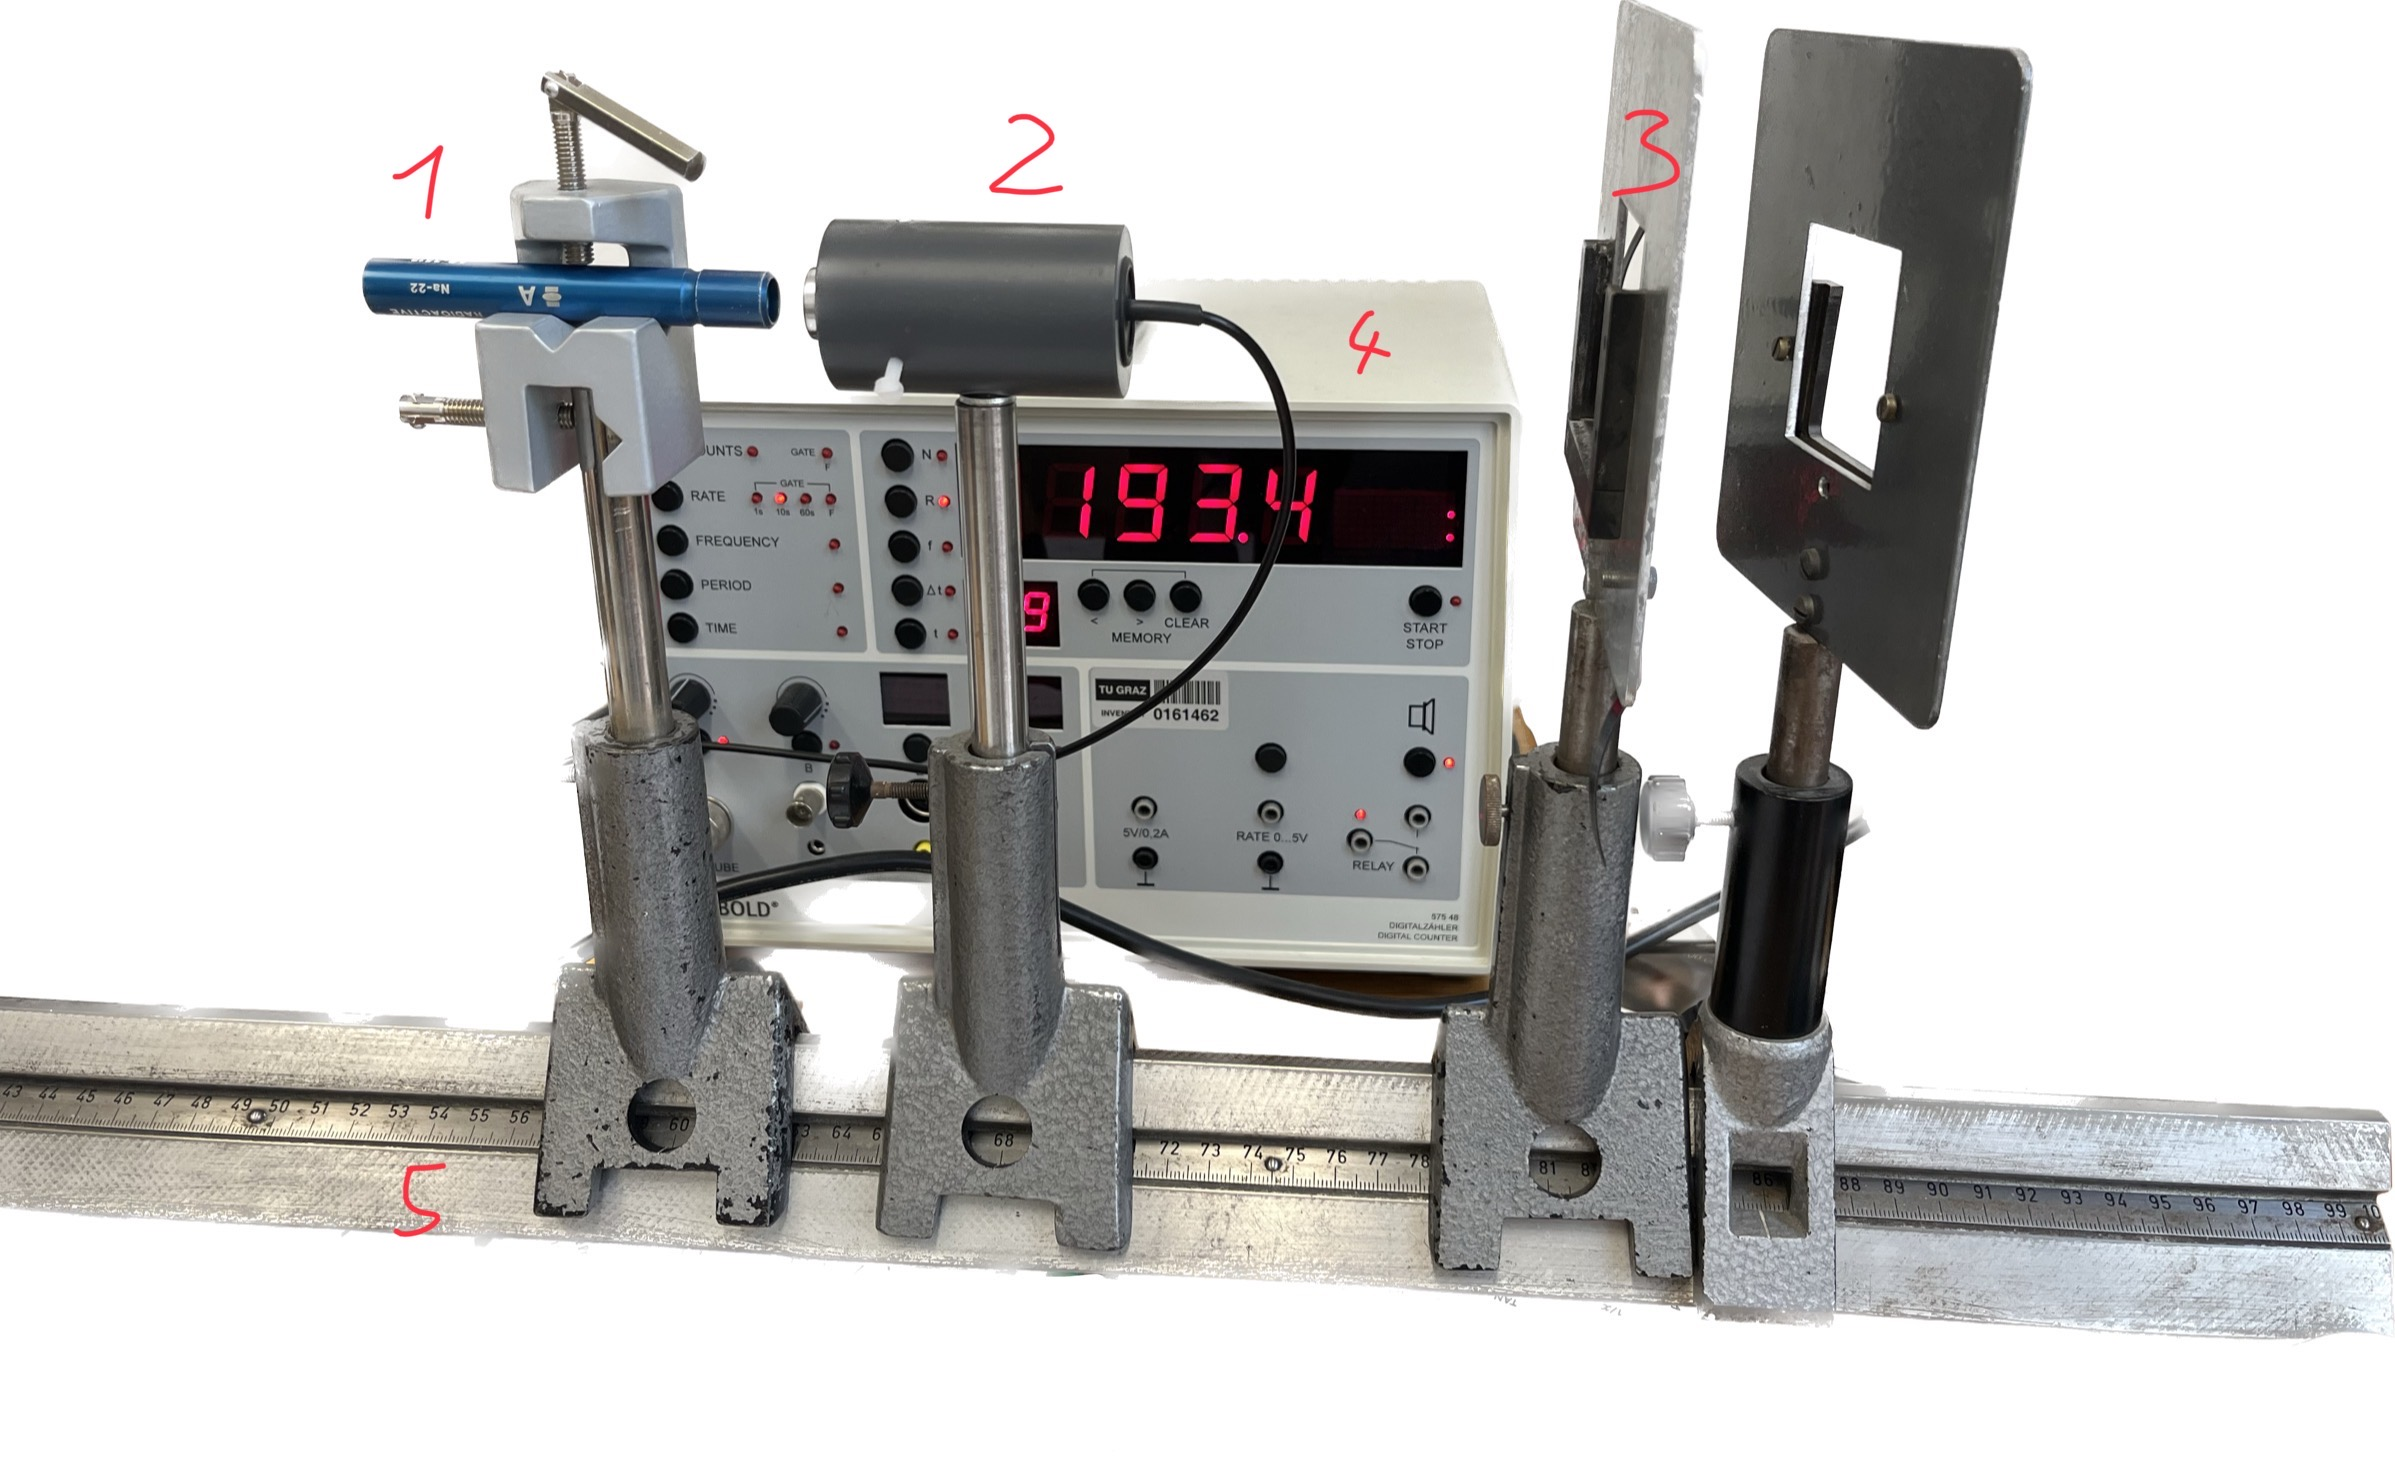
\includegraphics[width=0.8\textwidth]{./figures/digz.png}
	\end{center}
	\caption{Aufbau des Digitalzähler \\ 1 $\dots$ Halterung für radioaktive Quelle\\ 2 $\dots$ Zählrohr 
    \\3 $\dots$ Halterung um später das Aluminium zu Befestigen \\ 4 $\dots$ Digitalzähler 
    \\ 5 $\dots$ optische Bank um den Abstand zu variieren}
	\label{fig:digz}
    
\end{figure}










\newpage

\printbibliography
\listoffigures
\listoftables
\end{document}